\section{\moved{Hardware-efficient Inference}\added{: Details}}
\label{sec:hw_details}
\movednote{This section is moved from Section ``Hardware-efficient Inference'' of the previous version to the appendix.}

\subsection{\moved{Spike Generation via Direct FP16 Binary Parsing}}
\label{subsec:spike-gen-via-fp16-binary-parsing}

\moved{If the first 1 is found at position $k$ (counting from the most significant bit, $k = 1, 2, \ldots, 10$), the RMPA loop runs $k$ times and the corresponding threshold for the emitted spike is $\theta_k = (-1)^{S} \times 2^{E-15-k}.$ That is, position $k$ directly encodes the scaling factor $2^{-k}$ relative to the initial threshold, without any explicit computation. After the spike is emitted, the bit at position $k$ is cleared, and the LOD is applied to the updated mantissa in the next cycle to find the next 1. This process repeats until all cycles are exhausted or the mantissa becomes zero.}

\moved{We present an example of parsing the FP16 data of 1.4 in Figure~\ref{fig:spikes2fp16}.}

\begin{figure}[ht]
    \centering
    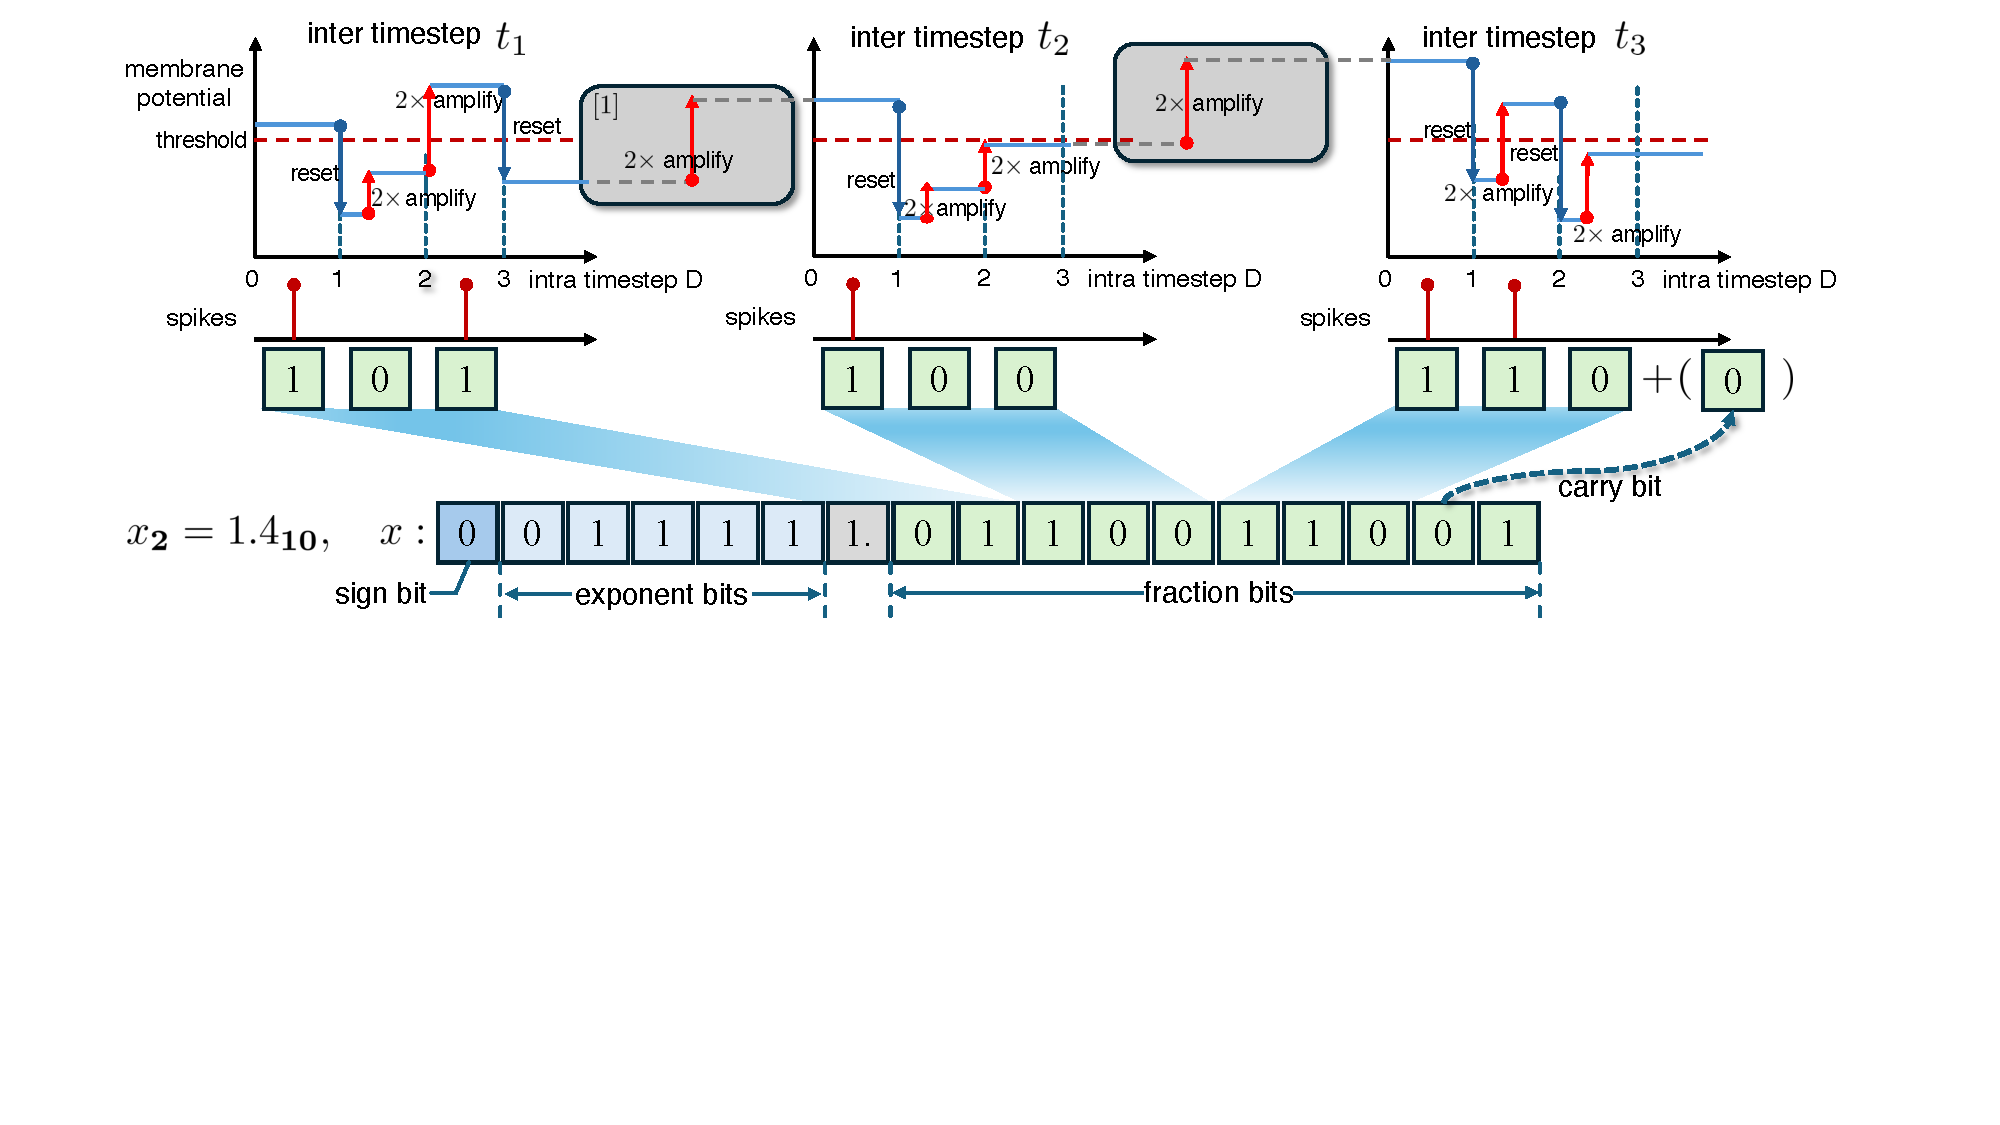
\includegraphics[width=1.0\linewidth]{Figs_new/figuers_1.pdf}
    \caption{Parsing the FP16 representation of 1.4 into spikes with D=T=3. The first inter-timestep emits the implicit 1 concatenated with the leading 2 mantissa bits at threshold $\theta = (-1)^{S} \times 2^{E-15-(D-1)}$; the second uses the LOD to locate the first 1 in the remaining 8 bits, reads D bits from that position as the spike value, and shifts the threshold accordingly. $^{[1]}$ The number of amplifications is not strictly one. It equals the bit-offset of the next leading 1 from the end of the current $T$-bit group.}
    \label{fig:spikes2fp16}
\end{figure}

\moved{We refer to $D$ as the intra-timestep spike dimension, which controls how many bits are emitted within a single timestep, and $T$ as the number of inter-timesteps, which controls how many successive timesteps are used to encode a given value. In the basic case ($D=1$), each timestep emits a 1-bit spike indicating whether the threshold is met. This paradigm further supports multi-bit spike emission by reading $D$ consecutive bits at a time, rather than a single bit. When $D > 1$, each spike is a $D$-bit unsigned integer ranging from 0 to $2^D - 1$, representing 0 to $2^D - 1$ times the corresponding threshold. For example, when $D=2$, 2 bits are read per timestep, encoding spike values in $\{0, 1, 2, 3\}$; when $D=3$, 3 bits are read, encoding values in $\{0, 1, \ldots, 7\}$. In the last timestep, an additional bit (i.e., the (D+1)-th bit) is read beyond the D-bit spike. This extra bit is then added to the D-bit spike value, treated as an unsigned integer, to perform a carry operation, which is equivalent to a round-half-up operation, and further improves encoding accuracy without introducing a separate rounding stage.}

\moved{At the hardware level, this intra-timestep expansion only requires widening the read window from 1 bit to $D$ bits; the LOD-based position finding and threshold determination remain unchanged. This multi-bit emission significantly increases the information density per timestep and is difficult to achieve in traditional ANN-to-SNN conversion algorithms, where each timestep is inherently limited to a binary fire-or-not decision.}

\subsection{\moved{Efficient Multiplication Under Spike Traces}}

\movedparagraph{Sign and Exponent.}
\moved{Given two FP16 operands $x$ and $w$, the sign and exponent of the product are computed in the standard manner. The output sign is obtained via a single XOR gate: $S_o = S_x \oplus S_w$, 
and the output exponent is $E_o = E_x + E_w - \text{bias}$, 
where $\text{bias} = 01111_2 = 15_{10}$. This requires only a 5-bit adder and a 6-bit subtractor, identical to a conventional FP16 multiplier. The key innovation lies entirely in how the mantissa product is computed, as described below.}

\begin{figure}[ht]
    \centering
    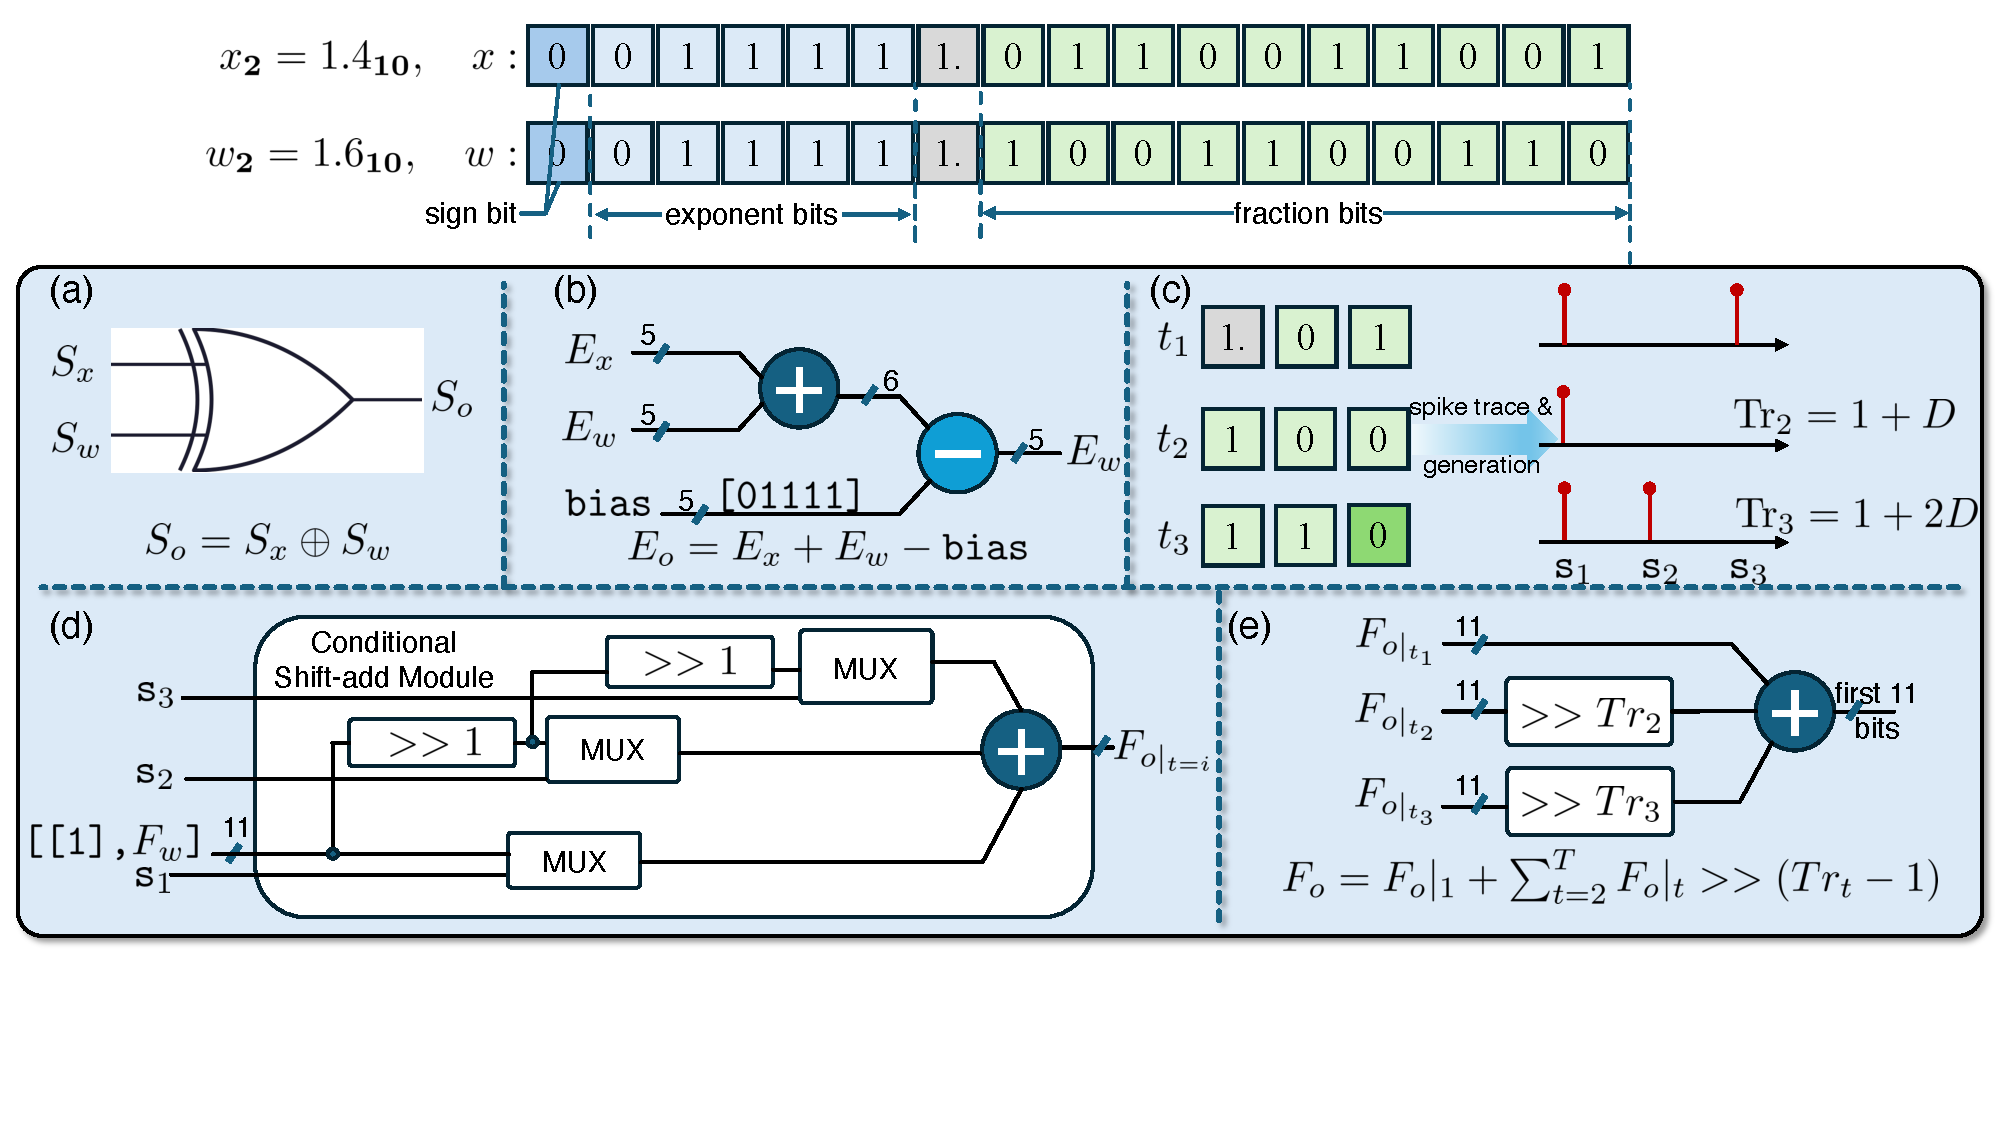
\includegraphics[width=1.0\linewidth]{Figs_new/figuers_2.pdf}
    \caption{Spike-driven FP16 multiplication. Sign, exponent, and mantissa of $x$ and $w$ are processed in parallel: \textbf{(a)} $S_o = S_x \oplus S_w$ via XOR; \textbf{(b)} $E_o = E_x + E_w - \text{bias}$ via a 5-bit adder and 6-bit subtractor; \textbf{(c)} the mantissa $F_x$ is decomposed into $T$ spikes $\{s_t\}$ with traces $\mathrm{Tr}_t = 1+(t-1)D$; \textbf{(d)} each partial product $F_{o}|_t = s_t \times F_w$ is computed by a Conditional Shift-add Module of MUXes and an adder tree, replacing the $11\times11$ multiplier array; \textbf{(e)} partial products are trace-aligned via right shifts and summed to form $F_o$, truncated to 11 bits.}
    \label{fig:calc}
\end{figure}

\movedparagraph{Mantissa Decomposition via Spike Traces.}
\moved{Let $F_x = 1.M_{x,1} M_{x,2} \cdots M_{x,10}$ denote the full mantissa of $x$ (including the implicit leading 1), and similarly $F_w$ for $w$. The spike generation process of the previous subsection decomposes $F_x$ into $T$ spike values $\{s_t\}_{t=1}^{T}$, each being a $D$-bit unsigned integer, with an associated trace value $\mathrm{Tr}_t$ that records the bit-position offset of the $t$-th spike relative to the binary point. Specifically, the first spike $s_1$ is composed of the implicit 1 together with the first $D-1$ mantissa bits, and the corresponding trace is $\mathrm{Tr}_1 = 1$. For subsequent timesteps $t \geq 2$, the LOD identifies the starting position of the next group, and $D$ consecutive bits are read as $s_t$. The trace value satisfies:
$
\mathrm{Tr}_t = 1 + (t-1) \times D,
$
when the mantissa bits are densely packed (i.e., no intervening zeros between groups). Under this decomposition, the mantissa can be reconstructed as $F_x = \sum_{t=1}^{T} s_t \times 2^{-(\mathrm{Tr}_t - 1)}.$ 
Substituting into the mantissa product yields:}
\begin{movedblock}
\begin{equation}\label{eq:mantissa_product}
F_o = F_x \times F_w = \sum_{t=1}^{T} \underbrace{(s_t \times F_w)}_{\triangleq\; F_{o}|_t} \times 2^{-(\mathrm{Tr}_t - 1)}.
\end{equation}
\end{movedblock}
\moved{This factorization reveals that the $11 \times 11$-bit mantissa multiplication is decomposed into $T$ smaller multiplications of a $D$-bit spike $s_t$ by the 11-bit mantissa $F_w$, followed by trace-aligned accumulation. Each per-timestep partial product $F_{o}|_t = s_t \times F_w$ is a $D$-bit $\times$ 11-bit multiplication, which can be efficiently realized by a Conditional Shift-add Module as illustrated in Figure~\ref{fig:spikes2fp16}(d). Let $s_t = \sum_{j=1}^{D} b_j \times 2^{D-j}$, where $b_j \in \{0,1\}$ are the individual bits of the $D$-bit spike. Then:}
\begin{movedblock}
\begin{equation}\label{eq:shift_add}
F_{o}|_t = s_t \times F_w = \sum_{j=1}^{D} b_j \times (F_w \gg (j-1)),
\end{equation}
\end{movedblock}
\moved{where $\gg$ denotes logical right shift. Each term $b_j \times (F_w \gg (j-1))$ is implemented by a multiplexer (MUX) controlled by $b_j$: when $b_j = 1$, the shifted value $F_w \gg (j-1)$ is selected; when $b_j = 0$, zero is selected. The $D$ selected values are then summed by an adder tree. This conditional shift-add structure replaces the combinatorial multiplier array with $D$ MUXes and a $(D-1)$-stage adder tree, significantly reducing the hardware area. Note that when $\text{spike} = 111$, the multiplication can be computed more efficiently by rewriting it as $1000 - 0001$, requiring only a single subtraction. A detailed derivation is provided in Appendix~\ref{sec:111}.}

\movedparagraph{Trace-aligned Temporal Accumulation.}
\moved{As shown in Figure~\ref{fig:calc}(e), the final mantissa is the trace-aligned sum of the $T$ partial products $F_{o}|_t$:}
\begin{movedblock}
\begin{equation}\label{eq:temporal_accum}
F_o = F_{o}|_1 + \sum_{t=2}^{T} F_{o}|_t \gg (\mathrm{Tr}_t - 1).
\end{equation}
\end{movedblock}
\moved{The right shift $\gg (\mathrm{Tr}_t - 1)$ aligns the $t$-th partial product to the correct bit position relative to the first partial product, and the final sum is truncated to the first 11 bits to produce the output mantissa.}

\section{Proof of Proposition~\ref{prop:rmpa-mtn-error-bound}}
\label{sec:error}
\movednote{The detailed derivation is moved to Section~\ref{sec:error-analysis} of the main text.}

\section{RMPA Example}
\label{sec:rmpa_example}
\movednote{The example is moved to Section~\ref{sec:method-ic} of the main text.}

\section{Energy Consumption Analysis\label{sec:energy}}

The energy savings achieved by ANN-to-SNN conversion stem from two primary sources: (1) replacing floating-point multiplication with lightweight addition operations, and (2) reducing bit-transmission cost between layers through the proposed spike encoding scheme. This section provides a detailed quantitative analysis of both aspects.

\subsection{Computational Energy Consumption}

Based on the proposed spike acquisition method, all multiplication operations $w \times x$ are fully decomposed into integer-level additions and bit-shift operations. For reference, prior work has established that FP32 multiplication consumes 3.7\,pJ and FP16 multiplication consumes 1.1\,pJ~\cite{energy}, as summarized in Table~\ref{tab:energy_operation}.

\begin{table}[htbp]
    \centering
    \caption{Energy Consumption of Common Hardware Operations}
    \label{tab:energy_operation}
    \begin{tabular}{ccc ccc}
        \toprule
        \multicolumn{2}{c}{\textbf{Integer Operation}}
        & \multicolumn{2}{c}{\textbf{Floating-Point Operation}}
        & \multicolumn{2}{c}{\textbf{Memory Access (64-bit)}} \\
        \cmidrule(lr){1-2} \cmidrule(lr){3-4} \cmidrule(lr){5-6}
        Operation   & Energy   & Operation    & Energy   & Memory       & Energy        \\
        \midrule
        8-bit Add   & 0.03\,pJ & 16-bit FAdd  & 0.4\,pJ  & 8\,KB Cache  & 10\,pJ        \\
        32-bit Add  & 0.1\,pJ  & 32-bit FAdd  & 0.9\,pJ  & 32\,KB Cache & 20\,pJ        \\
        8-bit Mult  & 0.2\,pJ  & 16-bit FMult & 1.1\,pJ  & 1\,MB Cache  & 100\,pJ       \\
        32-bit Mult & 3.1\,pJ  & 32-bit FMult & 3.7\,pJ  & DRAM         & 1.3--2.6\,nJ  \\
        \bottomrule
    \end{tabular}
\end{table}

Taking $T=2$, $D=3$ as a representative configuration (illustrated in Fig.~\ref{fig:calc} with $x=1.4$, $w=1.6$), the computation of $x \times w$ proceeds as follows.

\textbf{Step 1: Spike extraction from $x$.}
\begin{itemize}
    \item \textit{Cycle 1}: The spike is formed by the implicit leading 1 of the mantissa concatenated with the first $D-1=2$ fractional bits.
    \item \textit{Cycle 2}: The position $\mathrm{Tr}_2 $ of the first set bit among the remaining 8 mantissa bits is identified (here $\mathrm{Tr}_2=1 $), yielding a raw spike of \texttt{100}. A carry operation is then applied: the bit immediately following \texttt{100} is 1, so the spike is corrected to $\texttt{100}+1=\texttt{101}$.
    \item \textit{Remark}: Since the leading bit of each spike is always 1 by construction, it need not be transmitted explicitly; only the trailing $D-1$ bits are communicated, further reducing  bit-transmission cost between layers.
\end{itemize}

\textbf{Step 2: Exponent and sign processing.}
The sign bit of the result is obtained by XOR-ing the sign bits of $w$ and $x$. The exponent of the result is computed by summing the exponent fields of $w$ and $x$ and subtracting the bias of 15. The fractional part of $w$ is then shifted and accumulated in parallel according to the spike value of each cycle:
\begin{itemize}
    \item \texttt{spike = 101}: add the mantissa of $w$ and its right-shift by 2 bits.
    \item \texttt{spike = 100}: retain the mantissa of $w$ unchanged.
    \item \texttt{spike = 110}: add the mantissa of $w$ and its right-shift by 1 bit.
    \item \texttt{spike = 111}: compute the difference between the left-shifted mantissa and its right-shift by 2 bits (realizable via two's complement addition).
\end{itemize}

\textbf{Step 3: Cross-cycle accumulation.}
The fractional result from Cycle 1 is added to that of Cycle 2 right-shifted by $(\mathrm{Tr}_2 - 1)$ bits, accounting for any threshold scaling introduced by the carry operation. The final product $w \times x$ is assembled by concatenating the sign bit, the exponent, and the leading 11 bits of the accumulated mantissa.

\subsubsection*{Energy Estimation Basis}

Following established hardware scaling rules, energy consumption scales sub-linearly with operand width: doubling the bit-width typically increases energy by less than $2\times$~\cite{energy_scale}. On this basis, INT16 addition is estimated at 0.05--0.06\,pJ (conservatively taken as 0.06\,pJ), and sign-bit XOR is upper-bounded by INT8 addition at 0.03\,pJ.

\paragraph{First-Cycle Energy}

\begin{enumerate}[label=(\arabic*)]
    \item \textbf{Sign-bit XOR}: $0.03\,\text{pJ}$.
    \item \textbf{Exponent summation}: summing exponent bits and subtracting the bias consumes $0.06\,\text{pJ}$.
    \item \textbf{Spike--mantissa multiplication}:
    \begin{enumerate}[label=\textit{D=\arabic*}:, leftmargin=*]
        \item Retain mantissa directly; $0\,\text{pJ}$.
        \item With probability $1/2$ (\texttt{spike=10}): retain directly ($0\,\text{pJ}$); with probability $1/2$ (\texttt{spike=11}): one INT16 addition. Average: $(0+0.06)/2 = 0.03\,\text{pJ}$. Total with sign/exponent: $0.045\,\text{pJ}$.
        \item With probability $1/4$ (\texttt{spike=100}): $0\,\text{pJ}$; with probability $1/2$ (\texttt{spike=101,110}): one INT14 addition ($\approx0.06\,\text{pJ}$); with probability $1/4$ (\texttt{spike=111}): complement-based subtraction (estimated at $1.5\times$ INT addition). Average: $0.075\,\text{pJ}$.
    \end{enumerate}
    \item \textbf{Rounding}: one rounding operation on the mantissa at the end of each multiplication, $0.03\,\text{pJ}$, overlapped with Cycle 1.
\end{enumerate}

\paragraph{Subsequent-Cycle Energy ($T \geq 2$)}

\begin{enumerate}[label=(\arabic*)]
    \item \textbf{Leading-one detection}: locating the first set bit and recording offset $p$ is negligible; upper-bounded by INT8 addition at $0.03\,\text{pJ}$.
    \item \textbf{Spike--mantissa multiplication}: identical rules as Cycle 1; average energy is $0\,\text{pJ}$, $0.045\,\text{pJ}$, and $0.075\,\text{pJ}$ for $D=1,2,3$, respectively.
    \item \textbf{Cross-cycle accumulation}: right-shift by $(D+Tr_2-1)$ bits followed by addition. The maximum operand widths are INT24 ($D=2$) and INT25 ($D=3$), both truncated to INT16 addition: $0.03+0.06=0.09\,\text{pJ}$.
\end{enumerate}

The energy requirements for all subsequent cycles ($T>2$) are identical to those of Cycle 2. The total energy consumption in representative configurations $(T, D)$ is reported in Table~\ref{tab:power_consumption}.

\begin{table}[htbp]
    \centering
    \caption{Total Energy Consumption and Energy Ratio Relative to FP32 for Different $(T,\,D)$ Configurations (Unit: pJ)}
    \label{tab:power_consumption}
    \resizebox{0.5\textwidth}{!}{%
    \begin{tabular}{lccc}
        \toprule
        \textbf{Energy (pJ)} & $D{=}1$ & $D{=}2$ & $D{=}3$ \\
        \midrule
        $T{=}1$ & 0.090 & 0.210 & 0.330 \\
        $T{=}2$ & 0.165 & 0.330 & 0.495 \\
        $T{=}3$ & 0.195 & 0.390 & 0.585 \\
        \midrule
        FP16 (ANN) & \multicolumn{3}{c}{1.100} \\
        FP32 (ANN) & \multicolumn{3}{c}{3.700} \\
        \bottomrule
    \end{tabular}}
    \vspace{0.8em}
    \resizebox{0.5\textwidth}{!}{%
    \begin{tabular}{lccc}
        \toprule
        \makecell{\textbf{Energy Ratio} \\ \textbf{(SNN/FP32)}} & $T{=}1$ & $T{=}2$ & $T{=}3$ \\
        \midrule
        $D{=}1$ & 2.43\% & 5.68\% & 8.92\% \\
        $D{=}2$ & 4.46\% & 8.92\% & 13.38\% \\
        $D{=}3$ & 5.27\% & 10.54\% & 15.81\% \\
        \bottomrule
    \end{tabular}}
\end{table}

\begin{table}[htbp]
    \centering
    \caption{Total Energy Consumption and Energy Ratio for Different $(T,\,D)$ Configurations (Unit: pJ)}
    \label{tab:power_consumption_fp16}
    \resizebox{0.5\textwidth}{!}{%
    \begin{tabular}{lccc}
        \toprule
        \textbf{Energy (pJ)} & $D{=}1$ & $D{=}2$ & $D{=}3$ \\
        \midrule
        $T{=}1$ & 0.090 & 0.210 & 0.330 \\
        $T{=}2$ & 0.165 & 0.330 & 0.495 \\
        $T{=}3$ & 0.195 & 0.390 & 0.585 \\
        \midrule
        FP16 (ANN) & \multicolumn{3}{c}{1.100} \\
        FP32 (ANN) & \multicolumn{3}{c}{3.700} \\
        \bottomrule
    \end{tabular}}
    \vspace{0.8em}
    \resizebox{0.5\textwidth}{!}{%
    \begin{tabular}{lccc}
        \toprule
        \makecell{\textbf{Energy Ratio} \\ \textbf{(SNN/FP16)}} & $T{=}1$ & $T{=}2$ & $T{=}3$ \\
        \midrule
        $D{=}1$ & 8.18\% & 19.09\% & 30.00\% \\
        $D{=}2$ & 15.00\% & 30.00\% & 45.00\% \\
        $D{=}3$ & 17.73\% & 35.45\% & 53.18\% \\
        \bottomrule
    \end{tabular}}
\end{table}
 
\subsection{ bit-transmission cost between layers Evaluation}
 In traditional schemes, the  bit-transmission cost between layers depends on the data type: if the FP32 format is adopted, 32-bit data needs to be transmitted for each multiplication calculation; if the FP16 or BF16 format is adopted, 16-bit data needs to be transmitted for each multiplication calculation.
 The proposed  bit-transmission cost between layers consists of three parts: 1 bit sign information, 5 bit threshold information, $(D-1)$ bit spike information transmitted in the first cycle (the first bit defaults to 1 and can be omitted), and $(D-1+3)$ bit spike information transmitted in subsequent cycles (where the additional 3 bits are used to represent the threshold offset $\mathrm{Tr}_t$, with an upper limit of 8 bits: 000 for 1 and 111 for 8, and offsets exceeding 8 bits are directly ignored). The detailed transmission volume in different configurations is summarized in Table~\ref{tab:data_transmission}.

  \begin{table}[htbp]
    \centering
     \caption{ Bit-transmission Cost Between Layers Under Different Exponent Bit Widths and Parameter Configurations}
  \begin{tabular}{ccccc}
 
    \toprule
     \textbf{exp\_dim} & $\boldsymbol{D}$ & $\boldsymbol{T{=}1}$ & $\boldsymbol{T{=}2}$ & $\boldsymbol{T{=}3}$ \\
     \midrule
     \multirow{3}{*}{5} 
     & 1 & 6  & 9  & 15 \\
     & 2 & 7  & 11 & 18 \\
     & 3 & 8  & 13 & 21 \\
     \midrule
     \multirow{3}{*}{4} 
     & 1 & 5  & 8  & 14 \\
     & 2 & 6  & 10 & 17 \\
     & 3 & 7  & 12 & 20 \\
     \midrule
     FP32 (ANN)  & \multicolumn{4}{c}{32} \\
     FP16 or BF16 (ANN)  & \multicolumn{4}{c}{16} \\

     \bottomrule
   \end{tabular}
   
   \label{tab:data_transmission}
   \end{table}

 As can be seen in Table~\ref{tab:data_transmission}, the transmission bit width of the proposed scheme is significantly lower than that of traditional ANN schemes, thus further saving energy consumption in the data transmission process.

 

\section{Special Case: \texttt{spike} = \texttt{111}}
\label{sec:111}

\begin{figure}[htbp]
  \centering
  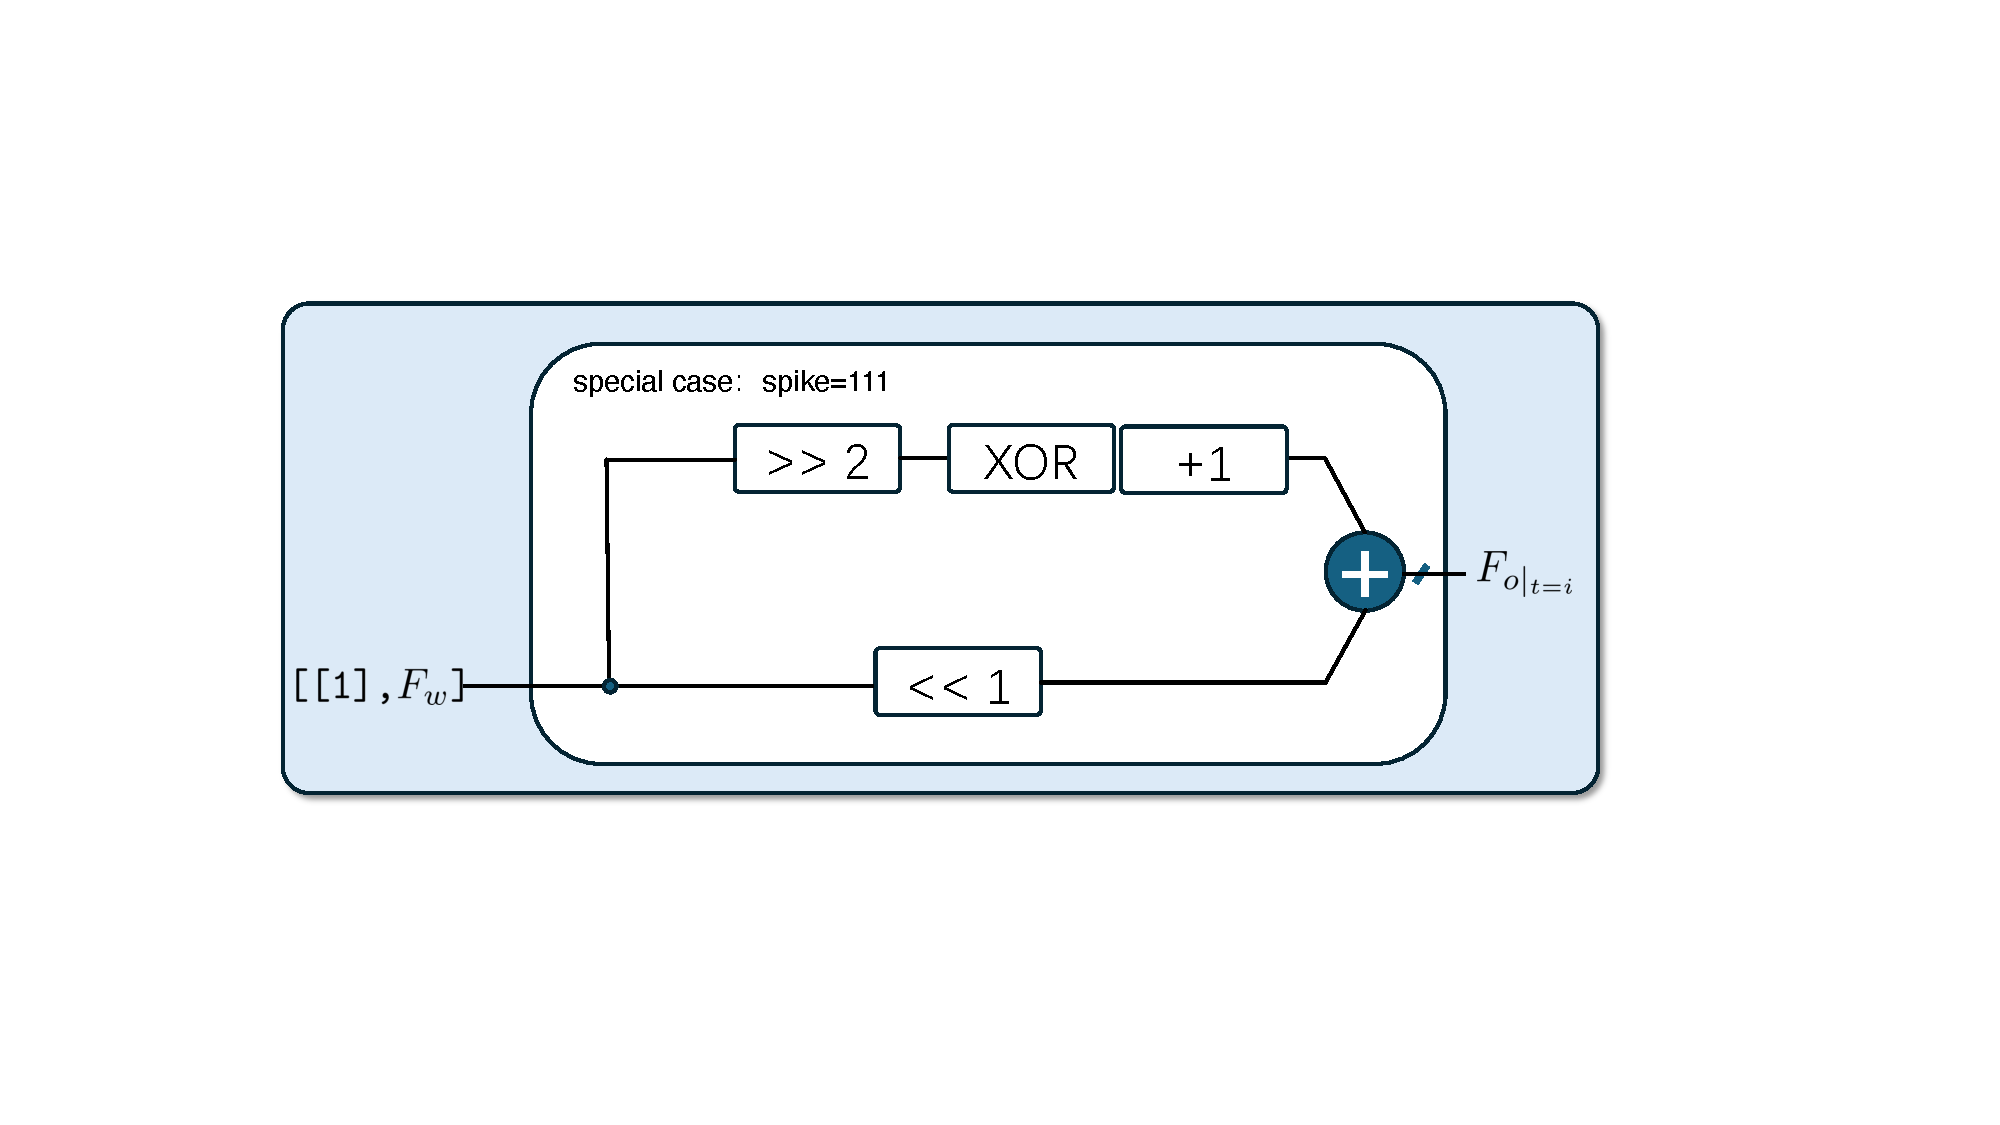
\includegraphics[width=0.6\textwidth]{Figs_new/figuersappendix.pdf}
  \caption{A special case for input spikes equals "\texttt{111}"}
  \label{fig:111}
\end{figure}

When $D = 3$ and \texttt{spike} $= \texttt{111}$, the naive shift-add formulation requires three terms:
\begin{equation}
    \begin{aligned}
        \relax[1, F_w] \cdot \texttt{111}_2 = [1, F_w] + ([1, F_w] \gg 1) + ([1, F_w] \gg 2),
    \end{aligned}
\end{equation}
which would naively require a two-stage adder tree. However, this case admits a more efficient decomposition. Observing that $\texttt{111}_2 = \texttt{1000}_2 - \texttt{0001}_2$, and noting that multiplication by $\texttt{1000}_2$ and $\texttt{0001}_2$ correspond to a left shift by 1 bit and a right shift by 2 bits, respectively (relative to the implicit leading bit), we obtain:
\[
[1, F_w] \cdot \texttt{111}_2 = ([1, F_w] \ll 1) - ([1, F_w] \gg 2),
\]
which requires only a single subtraction. In hardware, subtraction is implemented via two's complement addition: negating $[1, F_w] \gg 2$ is achieved by a bitwise complement followed by adding 1 (absorbed into the carry-in of the adder), yielding:
\[
[1, F_w] \cdot \texttt{111}_2 = ([1, F_w] \ll 1) + \overline{([1, F_w] \gg 2)},
\]
where $\ll$ and $\gg$ denote left and right logical shift respectively, and $\overline{(\cdot)}$ denotes the two's complement negation. As illustrated in Fig.~\ref{fig:111}, the datapath consists of a left-shift-by-1 unit on the lower path, a right-shift-by-2 unit followed by a two's complement unit on the upper path, and a single adder combining both results.

This decomposition ensures that, for all spike patterns with $D \leq 3$, each intra timestep computation requires \textbf{at most one adder}, with no case requiring more than a single addition or subtraction operation. The hardware overhead is therefore strictly bounded regardless of the spike value, confirming the area efficiency of the proposed design.

\section{Single-Step vs.\ Multi-Step Execution Modes}
\deletednote{Deleted: \texttt{\string\addcontentsline} line of the previous version.}

In ANN-to-SNN conversion, two execution modes can be distinguished based on the 
temporal scheduling strategy: \textit{single-step mode} and \textit{multi-step mode}.

\paragraph{Single-Step Mode.}
In single-step mode, the input data at each time step propagates through the entire 
network sequentially, layer by layer, before the next time step begins. That is, at 
time step $t$, the spike train is fully processed across all layers---from input to 
output---prior to the commencement of computation at time step $t+1$.

\paragraph{Multi-Step Mode.}
In multi-step mode, the execution order is transposed: for each layer, computations 
across all $T$ time steps are completed before proceeding to the next layer. 
Specifically, layer $\ell$ processes inputs for all time steps $t = 1, 2, \ldots, T$ 
and only then forwards the accumulated results to layer $\ell+1$.

\paragraph{Recommendation for RMPA.}
Even when RMPA is deployed without its hardware-level optimizations, we recommend 
adopting multi-step mode for the following reasons:

\begin{itemize}[leftmargin=*, nosep]
    \item \textbf{Hardware compatibility.} Multi-step mode aligns more naturally with 
    the dataflow patterns of contemporary hardware accelerators, where minimizing 
    memory access overhead is critical for sustained throughput.

    \item \textbf{Reduced weight reloading.} By completing all time steps within a 
    given layer before advancing to the next, multi-step mode eliminates the need to 
    repeatedly reload the same synaptic weights for each time step, thereby 
    significantly reducing memory bandwidth pressure.

    \item \textbf{Improved parallelism.} Multi-step mode naturally exposes 
    intra-layer parallelism across time steps, enabling more efficient utilization of 
    vectorized or batched computation resources.
\end{itemize}

\paragraph{Adapting RMPA for Single-Step Mode.}
If single-step mode is required by the deployment scenario, a minor modification to 
RMPA is necessary. Specifically, for the second and all subsequent time steps 
($t \geq 2$), when newly generated spike-driven data is forwarded to downstream 
layers, the membrane potential $m_\ell$ of layer $\ell$ must be updated by incorporating 
the incoming contribution scaled by $2^{i-1}$:
\begin{equation}
    \mathbf{m}_\ell(t) \leftarrow V_\ell(t) + 2^{i-1} \cdot \mathbf{I}_\ell(t), \qquad t \geq 2,
\end{equation}
where $\mathbf{I}_\ell(t)$ denotes the input increment arriving at layer $\ell$ at time step $t$, 
and $i$ is the number of RMPA loop. This scaling ensures that the accumulated membrane 
potential correctly reflects the appropriately amplified value.

\section{Ablation Study on Query Spiking Strategy}
\label{sec:query_ablation}
For the spiking conversion of Transformer models, this paper investigates the trade-off between computational efficiency and model accuracy in the treatment of the query (q) representation. By default, 
q is retained in floating-point form and excluded from spike conversion, while spiking conversion is applied exclusively to the key (k) and value(v). This design treats q as a weight-like parameter, which eliminates floating-point multiply-accumulate operations in the attention mechanism while preserving model accuracy. To assess the impact of this design choice, we conduct ablation experiments on whether to convert q into spikes, with results reported in Table~\ref{tab:query}.

\begin{table*}[htbp]
  \centering
  \caption{Experiments on ViT models under different $(T,D)$ settings. \texttt{q\_include} denotes the variant that also converts the query ($q$) into spikes (in addition to $k$ and $v$), while \texttt{Default} converts only $k$ and $v$.}
  \label{tab:query}
  \resizebox{\textwidth}{!}{
  \begin{tabular}{llcccccccccc}
    \toprule
    \multicolumn{1}{c}{\multirow{2}{*}{Task}} & 
    \multicolumn{1}{c}{\multirow{2}{*}{Model}} & 
    \multicolumn{1}{c}{\multirow{2}{*}{ANN}} & 
    \multicolumn{1}{c}{\multirow{2}{*}{$D$}} & 
    \multicolumn{3}{c}{Default} & 
    \multicolumn{3}{c}{q\_include} \\
    \cmidrule(lr){5-7} \cmidrule(lr){8-10}
    & & & & $T{=}1$ & $T{=}2$ & $T{=}3$ & $T{=}1$ & $T{=}2$ & $T{=}3$ \\
    
    \midrule
    \multirow{10}{*}{ImageNet-1K} 
    & \multirow{3}{*}{vit\_small\_patch16\_224} & \multirow{3}{*}{78.04}
    & 1 & 48.20 & 76.27 & 77.80 & 42.34 & 76.25 & 77.87 \\
    & & & 2 & 73.78 & 77.94 & 78.03 & 73.26 & 77.93 & 78.04 \\
    & & & 3 & 77.01 & 78.06 & 78.03 & 76.94 & 78.06 & 78.03 \\
    \cmidrule(lr){2-10}
    & \multirow{3}{*}{vit\_base\_patch16\_224} & \multirow{3}{*}{82.91}
    & 1 & 74.00 & 82.21 & 82.74 & 72.37 & 82.17 & 82.73 \\
    & & & 2 & 80.89 & 82.77 & 82.89 & 80.71 & 82.76 & 82.87 \\
    & & & 3 & 82.41 & 82.87 & 82.91 & 82.43 & 82.87 & 82.92 \\
    \cmidrule(lr){2-10}
    & \multirow{3}{*}{vit\_large\_patch16\_224} & \multirow{3}{*}{84.88}
    & 1 & 80.89 & 84.46 & 84.79 & 80.26 & 84.43 & 84.79 \\
    & & & 2 & 84.03 & 84.80 & 84.89 & 83.96 & 84.81 & 84.89 \\
    & & & 3 & 84.45 & 84.89 & 84.88 & 84.41 & 84.89 & 84.88 \\
    
    \midrule
    
    \multirow{15}{*}{MMLU}
    & \multirow{3}{*}{qwen3\_0.6b\_base} & \multirow{3}{*}{52.41}
    & 1 & 29.06 & 50.29 & 52.11 & 25.58 & 49.47 & 52.31 \\
    & & & 2 & 45.85 & 52.55 & 52.56 & 43.40 & 52.24 & 52.73 \\
    & & & 3 & 51.08 & 52.60 & 52.49 & 50.11 & 52.60 & 52.60 \\
    \cmidrule(lr){2-10}
    & \multirow{3}{*}{qwen3\_1.7b\_base} & \multirow{3}{*}{62.61}
    & 1 & 41.59 & 60.80 & 62.37 & 31.94 & 60.12 & 62.47 \\
    & & & 2 & 57.83 & 62.42 & 62.53 & 55.62 & 62.34 & 62.78 \\
    & & & 3 & 60.87 & 62.26 & 62.50 & 60.93 & 62.63 & 62.56 \\
    \cmidrule(lr){2-10}
    & \multirow{3}{*}{qwen3\_4b\_base} & \multirow{3}{*}{72.90}
    & 1 & 57.58 & 72.34 & 72.70 & 43.85 & 71.57 & 72.72 \\
    & & & 2 & 69.29 & 72.75 & 73.10 & 67.40 & 72.62 & 73.07 \\
    & & & 3 & 72.21 & 72.92 & 73.04 & 71.85 & 73.00 & 73.04 \\
    \cmidrule(lr){2-10}
    & \multirow{3}{*}{qwen3\_8b\_base} & \multirow{3}{*}{76.85}
    & 1 & 65.26 & 76.13 & 76.86 & 54.42 & 75.97 & 76.51 \\
    & & & 2 & 74.88 & 76.71 & 76.78 & 73.06 & 76.59 & 76.81 \\
    & & & 3 & 76.45 & 76.90 & 76.81 & 75.99 & 76.81 & 76.73 \\
    \cmidrule(lr){2-10}
    & \multirow{3}{*}{qwen3\_14b\_base} & \multirow{3}{*}{80.47}
    & 1 & 70.70 & 79.73 & 80.39 & 62.08 & 79.58 & 80.37 \\
    & & & 2 & 78.63 & 80.47 & 80.45 & 77.43 & 80.42 & 80.65 \\
    & & & 3 & 80.37 & 80.49 & 80.49 & 79.83 & 80.40 & 80.44 \\

    \bottomrule
  \end{tabular}
  }
\end{table*}

\section{Additional Experimental Results on ImageNet-1K}\label{overall_imagenet}

This section presents comprehensive experimental results of our SNN conversion framework on the ImageNet-1K dataset across various models, including EVA02, ViT, ResNet, and VGG. We report accuracy in different timesteps \(T\) and spike dimensions \(D\) in table~\ref{tab:appendix_imagenet}. The ANN baseline accuracy is provided for reference.

\begin{table*}[htbp]
\centering
\caption{Accuracy (\%) on ImageNet-1K Dataset under Different $T$ and $D$ Settings}
\label{tab:appendix_imagenet}
\begin{minipage}{0.48\textwidth}
\centering
\begin{tabular}{lcccc}
\toprule
\textbf{Model} & $T=1$ & $T=2$ & $T=3$ & \textbf{ANN} \\
\midrule
\multicolumn{5}{l}{\textbf{eva02\_tiny\_patch14\_336}} \\
$d=1$ & 73.26 & 80.11 & 80.53 & 80.62 \\
$d=2$ & 78.82 & 80.60 & 80.65 \\
$d=3$ & 80.19 & 80.63 & 80.61 \\
\midrule
\multicolumn{5}{l}{\textbf{eva02\_small\_patch14\_336}} \\
$d=1$ & 80.18 & 85.22 & 85.68 & 85.73 \\
$d=2$ & 84.54 & 85.74 & 85.75 \\
$d=3$ & 85.45 & 85.70 & 85.73 \\
\midrule
\multicolumn{5}{l}{\textbf{eva02\_base\_patch14\_448}} \\
$d=1$ & 81.53 & 87.85 & 88.25 & 88.26 \\
$d=2$ & 86.88 & 88.28 & 88.26 \\
$d=3$ & 88.00 & 88.27 & 88.26 \\
\midrule
\multicolumn{5}{l}{\textbf{eva02\_large\_patch14\_448}} \\
$d=1$ & 85.66 & 89.32 & 89.57 & 89.63 \\
$d=2$ & 88.88 & 89.60 & 89.63 \\
$d=3$ & 89.46 & 89.63 & 89.63 \\
\midrule
\multicolumn{5}{l}{\textbf{eva\_giant\_patch14\_336}} \\
$d=1$ & 88.65 & 89.41 & 89.57 & 89.62 \\
$d=2$ & 89.27 & 89.56 & 89.60 \\
$d=3$ & 89.47 & 89.58 & 89.62 \\
\bottomrule
\end{tabular}
\end{minipage}
\hfill
\begin{minipage}{0.48\textwidth}
\centering
\begin{tabular}{lcccc}
\toprule
\textbf{Model} & $T=1$ & $T=2$ & $T=3$ & \textbf{ANN} \\
\midrule
\multicolumn{5}{l}{\textbf{vit\_small\_patch16\_224}} \\
$d=1$ & 48.20 & 76.27 & 77.80 & 78.04 \\
$d=2$ & 73.78 & 77.94 & 78.03 \\
$d=3$ & 77.01 & 78.06 & 78.03 \\
\midrule
\multicolumn{5}{l}{\textbf{vit\_base\_patch16\_224}} \\
$d=1$ & 74.00 & 82.21 & 82.74 & 82.91 \\
$d=2$ & 80.89 & 82.77 & 82.89 \\
$d=3$ & 82.41 & 82.87 & 82.91 \\
\midrule
\multicolumn{5}{l}{\textbf{vit\_large\_patch16\_224}} \\
$d=1$ & 80.89 & 84.46 & 84.79 & 84.88 \\
$d=2$ & 84.03 & 84.80 & 84.89 \\
$d=3$ & 84.45 & 84.89 & 84.88 \\
\midrule
\multicolumn{5}{l}{\textbf{resnet34}} \\
$d=1$ & 20.23 & 72.45 & 75.83 & 76.09 \\
$d=2$ & 66.59 & 76.08 & 76.12 \\
$d=3$ & 74.81 & 76.13 & 76.09 \\
\midrule
\multicolumn{5}{l}{\textbf{vgg16}} \\
$d=1$ & 49.82 & 68.86 & 70.97 & 71.12 \\
$d=2$ & 65.25 & 70.94 & 71.10 \\
$d=3$ & 69.72 & 71.08 & 71.12 \\
\bottomrule
\end{tabular}
\end{minipage}
\end{table*}

\section{Experimental Results on CIFAR datasets}\label{overall_cifars}

\begin{figure}[ht!]
    \centering
    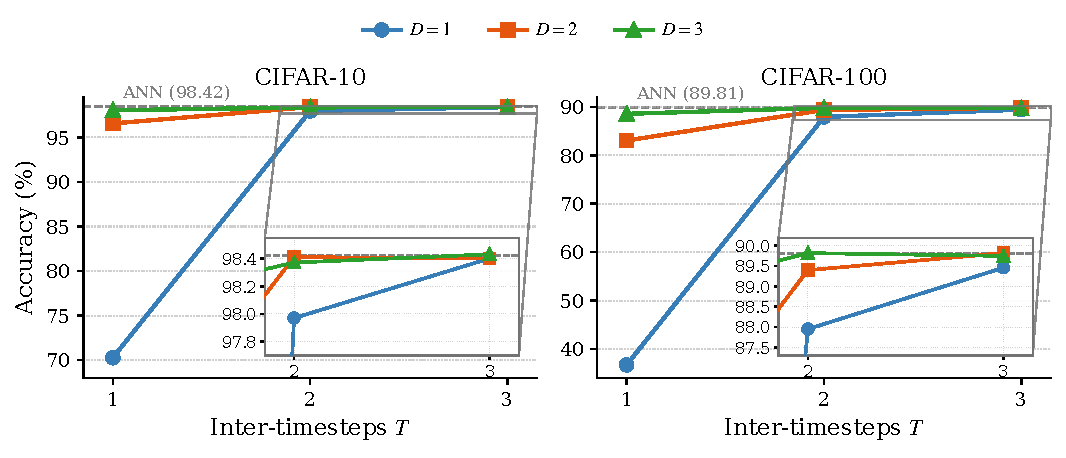
\includegraphics[width=1\linewidth]{Figs_new/cifar_accuracy.pdf}
    \caption{Test accuracy of ViT-S on CIFAR-10 (left) and CIFAR-100 (right) under different settings of  $T$ and $D$.}
    \label{fig:cifar}
\end{figure}

We evaluate the converted ViT-S model in CIFAR tasks under different combinations of parameters and report the post-conversion accuracy in figure~\ref{fig:cifar}.

For CIFAR-10, with \(D=1\), our method achieves \textbf{98.40\%} accuracy at \(T=3\), closely matching the ANN baseline (98.42\%) while requiring only 3 timesteps. Remarkably, even at \(T=2\), the accuracy reaches 97.97\%, with a negligible drop of 0.45\%. For CIFAR-100, our method attains \textbf{89.46\%} at \(T=3\) and 87.95\% at \(T=2\), again approaching the baseline of the ANN of 89.81\%.

We further observe that deeper networks enable faster convergence. With \(D=3\), the SNN on CIFAR-10 already reaches 98.05\% at \(T=1\) and saturates at 98.37\% for \(T=3\), effectively matching the ANN. Similarly, on CIFAR-100, \(D=3\) yields 88.59\% at \(T=1\) and 89.82\% at \(T=2\), narrowing the gap to within 0.06\% of the ANN. These results demonstrate that our method achieves almost lossless conversion with as few as \(T=2\) timesteps, and deeper architectures further reduce the required latency. 

\section{Experimental Results on MMLU Benchmark}\label{overall_mmlu}

\begin{figure}[ht!]
    \centering
    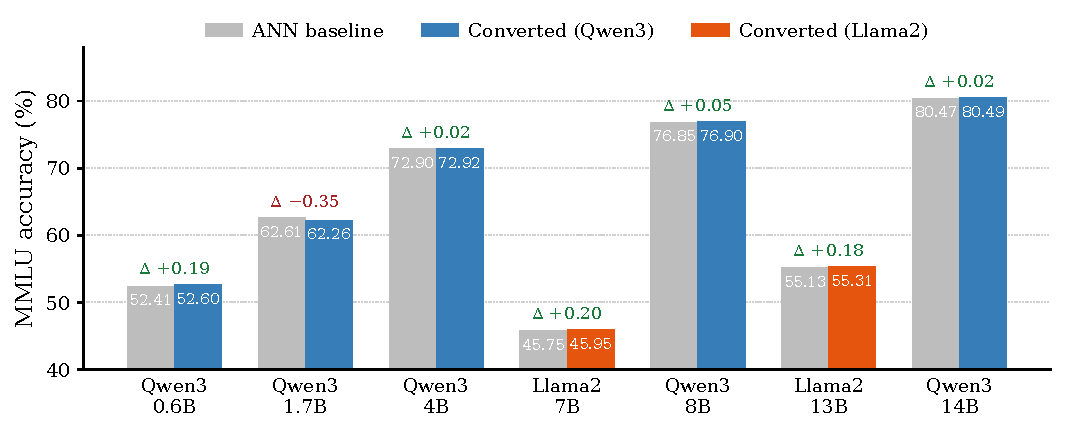
\includegraphics[width=0.7\linewidth]{Figs_new/mmlu_comparison.pdf}
    \caption{Conversion results on MMLU for different models}
    \label{fig:mmlu}
\end{figure}

The Qwen3\cite{qwen3} and Llama2\cite{llama2} series models are evaluated on the  MMLU benchmark in this work. We perform comprehensive evaluations on this key NLP benchmark, and the corresponding results are shown in figure~\ref{fig:mmlu}.

\clearpage
\section{Additional Experimental Results of LLaMA2-7B and LLaMA2-13b}\label{overall_llama}

This section presents comprehensive experimental results of our SNN conversion framework on various NLP tasks for the LLaMA2-7B and LLaMA2-13B models in table~\ref{tab:appendix_llama}. We report accuracy in different timesteps \(T\) and spike dimensions \(D\). The ANN baseline accuracy is provided for reference.

\begin{table*}[htbp!]
\centering
\caption{Accuracy (\%) of LLaMA2-7B and LLaMA2-13B on NLP Tasks under Different $T$ and $D$ Settings}
\label{tab:appendix_llama}
\resizebox{0.8\textwidth}{!}{
\begin{tabular}{lccccclcccc}
\toprule
& \multicolumn{4}{c}{\textbf{LLaMA2-7B}} & & \multicolumn{4}{c}{\textbf{LLaMA2-13B}} \\
\cmidrule(lr){2-5} \cmidrule(lr){7-10}
\textbf{Task} & $$T{=}1$$ & $$T{=}2$$ & $$T{=}3$$ & ANN & & $$T{=}1$$ & $$T{=}2$$ & $$T{=}3$$ & ANN \\
\midrule
\multicolumn{10}{l}{\textbf{MMLU}} \\
$$d{=}1$$ & 26.90 & 43.88 & 45.93 & 45.75 & & 33.76 & 53.62 & 54.99 & 55.13 \\
$$d{=}2$$ & 39.97 & 45.67 & 45.73 &  & & 51.40 & 55.05 & 55.23 &  \\
$$d{=}3$$ & 44.92 & 45.95 & 45.93 &  & & 54.15 & 55.31 & 55.14 & \\
\midrule
\multicolumn{10}{l}{\textbf{PIQA-norm}} \\
$$d{=}1$$ & 72.14 & 79.11 & 78.56 & 78.45 & & 74.32 & 80.09 & 80.52 & 80.52 \\
$$d{=}2$$ & 77.37 & 78.73 & 78.84 &  & & 79.60 & 80.69 & 80.25 &  \\
$$d{=}3$$ & 78.78 & 78.67 & 78.51 & & & 80.25 & 80.58 & 80.47 &  \\
\midrule
\multicolumn{10}{l}{\textbf{ARC-Challenge norm}} \\
$$d{=}1$$ & 33.19 & 44.88 & 45.48 & 45.73 & & 39.76 & 48.55 & 48.55 & 48.89 \\
$$d{=}2$$ & 43.60 & 45.48 & 45.65 &  & & 47.78 & 48.72 & 48.38 &  \\
$$d{=}3$$ & 46.16 & 45.65 & 45.99 &  & & 49.40 & 49.15 & 48.55 & \\
\midrule
\multicolumn{10}{l}{\textbf{ARC-Easy norm}} \\
$$d{=}1$$ & 58.33 & 73.61 & 74.75 & 74.87 & & 66.79 & 75.93 & 76.60 & 76.56 \\
$$d{=}2$$ & 72.26 & 73.99 & 74.54 &  & & 75.51 & 76.26 & 76.47 &  \\
$$d{=}3$$ & 73.82 & 74.75 & 74.66 &  & & 75.80 & 76.47 & 76.43 & \\
\midrule
\multicolumn{10}{l}{\textbf{Winogrande norm}} \\
$$d{=}1$$ & 60.38 & 69.38 & 69.46 & 69.38 & & 62.67 & 71.90 & 71.90 & 72.22 \\
$$d{=}2$$ & 67.01 & 69.53 & 69.30 & & & 71.43 & 72.53 & 72.22 &  \\
$$d{=}3$$ & 67.56 & 69.06 & 69.46 &  & & 70.56 & 72.14 & 72.53 &  \\
\midrule
\multicolumn{10}{l}{\textbf{HellaSwag norm}} \\
$$d{=}1$$ & 65.61 & 75.72 & 76.30 & 76.28 & & 66.05 & 79.04 & 79.55 & 79.71 \\
$$d{=}2$$ & 74.65 & 76.25 & 76.18 &  & & 78.57 & 79.63 & 79.71 &  \\
$$d{=}3$$ & 75.77 & 76.18 & 76.25 &  & & 79.23 & 79.69 & 79.72 & \\
\bottomrule
\end{tabular}
}
\end{table*}
\clearpage
\section{MMLU Results of Qwen3 Series Models}\label{overall_qwen3}
This section supplements the accuracy of the MMLU task of the Qwen3 series with different timesteps \(T\) and spike dimensions \(D\) in table~\ref{tab:appendix_qwen3_mmlu}, with the original ANN accuracy provided as the baseline reference.

\begin{table*}[htbp!]
\centering
\caption{MMLU Accuracy (\%) of Qwen3 Series Models under Different $T$ and $D$ Settings}
\label{tab:appendix_qwen3_mmlu}
\small
\begin{tabular}[t]{lcccc}
\toprule
\textbf{Model} & $T{=}1$ & $T{=}2$ & $T{=}3$ & \textbf{ANN} \\
\midrule
\multicolumn{5}{l}{\textbf{qwen3-0.6b-base}} \\
$d{=}1$ & 29.06 & 50.29 & 52.11 & 52.41 \\
$d{=}2$ & 45.85 & 52.55 & 52.56 & \\
$d{=}3$ & 51.08 & 52.60 & 52.49 & \\
\midrule
\multicolumn{5}{l}{\textbf{qwen3-1.7b-base}} \\
$d{=}1$ & 41.59 & 60.80 & 62.37 & 62.61 \\
$d{=}2$ & 57.83 & 62.42 & 62.53 & \\
$d{=}3$ & 60.87 & 62.26 & 62.50 & \\
\midrule
\multicolumn{5}{l}{\textbf{qwen3-4b-base}} \\
$d{=}1$ & 57.58 & 72.34 & 72.70 & 72.90 \\
$d{=}2$ & 69.29 & 72.75 & 73.10 & \\
$d{=}3$ & 72.21 & 72.92 & 73.04 & \\
\bottomrule
\end{tabular}
\hspace{2.5em}
\begin{tabular}[t]{lcccc}
\toprule
\textbf{Model} & $T{=}1$ & $T{=}2$ & $T{=}3$ & \textbf{ANN} \\
\midrule
\multicolumn{5}{l}{\textbf{qwen3-8b-base}} \\
$d{=}1$ & 65.26 & 76.13 & 76.86 & 76.85 \\
$d{=}2$ & 74.88 & 76.71 & 76.78 & \\
$d{=}3$ & 76.45 & 76.90 & 76.81 & \\
\midrule
\multicolumn{5}{l}{\textbf{qwen3-14b-base}} \\
$d{=}1$ & 70.70 & 79.73 & 80.39 & 80.47 \\
$d{=}2$ & 78.63 & 80.47 & 80.45 & \\
$d{=}3$ & 80.37 & 80.49 & 80.49 & \\
\bottomrule
\end{tabular}
\end{table*}

\section{Support for More Formats\label{sec:fp8_int4}}

We emphasize that based on ANN2SNN, this framework can further combine with model quantization strategies, bringing additional benefits in data movement and energy consumption. The two complement each other, making it more friendly for edge AI. For this reason, we explored the efficiency and performance comparison of models under extreme quantization conditions (INT4). Following the energy estimation method for ultra-low bit operations described in~\cite{liu2020birealnet,qin2020binary}, we set the energy consumption of single-bit logic gate operations to 3.75\,fJ and calculated the efficiency of the quantized model under INT4 or FP8 conditions and the conversion model under the PRIME framework (as shown in Table~\ref{tab:fp8_prime},\ref{tab:int4_prime}).

\subsection{FP8 Format}

Table~\ref{tab:fp8_prime} summarizes the energy consumption and bit-transmission cost after PRIME conversion on FP8 operands.Table~\ref{tab:qwen3_fp8_mmlu} reports the MMLU accuracy of Qwen3-0.6B in FP8 format before and after PRIME conversion.

\begin{table*}[htbp]
  \centering
  \scriptsize
  \caption{Energy and bit-transmission cost of FP8 format after PRIME conversion.}
  \label{tab:fp8_prime}
  \resizebox{1\textwidth}{!}{
  \begin{tabular}{lcccc}
    \toprule
    & Energy (pJ) & Energy Ratio (vs.\ FP8) & Transmission Bits & Transmission Ratio (vs.\ FP8) \\
    \midrule
    T1D1 & 0.0375  & 13.39\%   & 5 & 62.50\%  \\
    T1D2 & 0.04875 & 17.41\%   & 6 & 75.00\%  \\
    T2D1 & 0.07125 & 25.45\%   & 6 & 75.00\%  \\
    T2D2 & 0.09375 & 33.48\%   & 8 & 100.00\% \\
    FP8  & 0.28    & 100.00\%  & 8 & 100.00\% \\
    \bottomrule
  \end{tabular}
  }
\end{table*}

\begin{table*}[htbp]
  \centering
  \scriptsize
  \caption{MMLU accuracy of Qwen3-0.6B-FP8 before and after PRIME conversion.}
  \label{tab:qwen3_fp8_mmlu}
  \resizebox{0.4\textwidth}{!}{
  \begin{tabular}{lc}
    \toprule
    Config & MMLU Acc (\%) \\
    \midrule
    Pure FP8 (Baseline\_a8w8) & 26.78 \\
    \midrule
    T1D1 & 16.38 \\
    T1D2 & 23.84 \\
    T2D1 & 25.76 \\
    T2D2 & 26.66 \\
    \bottomrule
  \end{tabular}
  }
\end{table*}

\subsection{INT4 Format}

Table~\ref{tab:int4_prime} summarizes the energy and bit-transmission analysis for INT4 operands.Table~\ref{tab:flatquant_prime_llama2} reports the accuracy of LLaMA2-7B under FlatQuant W4A4 quantization and further PRIME conversion.

\begin{table*}[htbp]
  \centering
  \scriptsize
  \caption{Energy and bit-transmission cost of INT4 format after PRIME conversion.}
  \label{tab:int4_prime}
  \resizebox{1\textwidth}{!}{
  \begin{tabular}{lcccc}
    \toprule
    & Energy (pJ) & Energy Ratio (vs.\ INT4) & Transmission Bits & Transmission Ratio (vs.\ INT4) \\
    \midrule
    T1D1 & 0.01125  & 22.50\%   & 3 & 75.00\%  \\
    T1D2 & 0.016875 & 33.75\%   & 4 & 100.00\% \\
    T2D1 & 0.0375   & 75.00\%   & 4 & 100.00\% \\
    INT4 & 0.05     & 100.00\%  & 4 & 100.00\% \\
    \bottomrule
  \end{tabular}
  }
\end{table*}

\begin{table*}[htbp]
  \centering
  \scriptsize
  \caption{Accuracy comparison of FlatQuant W4A4 and further PRIME conversion on LLaMA2-7B.}
  \label{tab:flatquant_prime_llama2}
  \resizebox{\textwidth}{!}{
  \begin{tabular}{lcccccccc}
    \toprule
    & PPL(wiki) & PPL(c4) & ARC\_c & ARC\_e & Hella & LAMB & PIQA & Wino \\
    \midrule
    FlatQuant W4A4 & 5.69 & 7.62  & 44.37 & 73.11 & 74.80 & 72.27 & 77.86 & 67.88 \\
    PRIME T1D1     & 9.50 & 13.79 & 35.49 & 63.68 & 64.62 & 62.62 & 75.19 & 62.04 \\
    PRIME T1D2     & 6.15 & 8.33  & 40.44 & 69.70 & 72.52 & 70.64 & 77.20 & 66.46 \\
    PRIME T2D1     & 6.17 & 8.38  & 43.00 & 70.03 & 72.58 & 70.06 & 76.44 & 64.25 \\
    \bottomrule
  \end{tabular}
  }
\end{table*}

\section{Limitations}
Our current evaluation is simulation-based and does not include silicon measurements. However, since all underlying primitives (bit-shift, integer addition, and leading-one detection) are naively supported by standard digital logic, the proposed neuron dynamics require no custom analog or mixed-signal circuitry. Physical implementation is therefore a natural next step, which we leave to our future work.